\documentclass[a4paper, oneside]{memoir}% Document class
\usepackage[a4paper]{geometry}			% Margins
\usepackage{lmodern}
\usepackage{graphicx}
\usepackage{float}
\usepackage{listings}
\usepackage[small,compact]{titlesec}	% No 'chapter' in chapter headings.
\graphicspath{{Media/}}					% Directory that holds images.

\titleformat{\chapter}[hang]
{\normalfont\Large\bfseries}{\thechapter}{1em}{\Large}
\titlespacing{\chapter}{0pt}{*0}{*1}

\titleformat{\chapter}{\Huge\bfseries}{\thechapter}{1em}{}
\titleformat{\section}{\LARGE\bfseries}{\thesection}{1em}{}
\titleformat{\subsection}{\Large\bfseries}{\thesubsection}{1em}{}
\titleformat{\subsubsection}{\normalsize\bfseries}{\thesubsubsection}{1em}{}


\author{
  Erik Sidelmann Jensen\\
  \texttt{ejens11@student.aau.dk}
  \and
  Lasse Vang Gravesen\\
  \texttt{lgrave11@student.aau.dk}
  \and
  Dennis Jakobsen\\
  \texttt{djakob11@student.aau.dk}  
}

\title{Web Intelligence - Crawler Miniproject}
\date{}

\begin{document}
	\clearpage\maketitle
	\thispagestyle{empty}
	
	\chapter{Crawler Miniproject}
	\section{Crawler}
	Our crawler works as follows:
	
	The Crawler class has a frontier, a list of visited urls, a dictionary of hashes for the visited urls to be used for checking content equality. It also uses a custom WebClient that has a timeout value along with a database for inserting crawled items into.
	
	The Crawler is started by setting a list of seed urls, which are added to the frontier. Then the amount of items to be crawled is set and these are run in a loop until it is complete.
	
	It gets the next url to be crawled and if it passes politeness checks that is if the page to be crawled on the url is allowed by the `robots.txt' file and it also checks if the that url is not in the list of visited urls.
	
	It tries to download the content of the url, and if it fails it just adds the url to the list of visited urls and sleeps for second.
	
	If the content downloaded correctly, it will check if an equal already exists in the system using shingling with sketches and Jaccard similarity, if it has an equal it adds it to the list of visited urls and sleeps and then `continue' the loop.
	
	If it does not have an equal it adds it to the visited urls, it extracts the urls in the content, normalizes them and if the frontier has not met the size limit it will check if it passes the checks and if it does it will add it to the frontier. It also adds the Html and Url to the database for later use. 
	
	The architecture is somewhat similar to the architecture used by Bo in his slides, though there are some differences specifically with the `robots.txt' check in that it does that check for each url it visits instead of performing the check before adding it to the frontier.
	
	\begin{figure}[H]
	\centering
	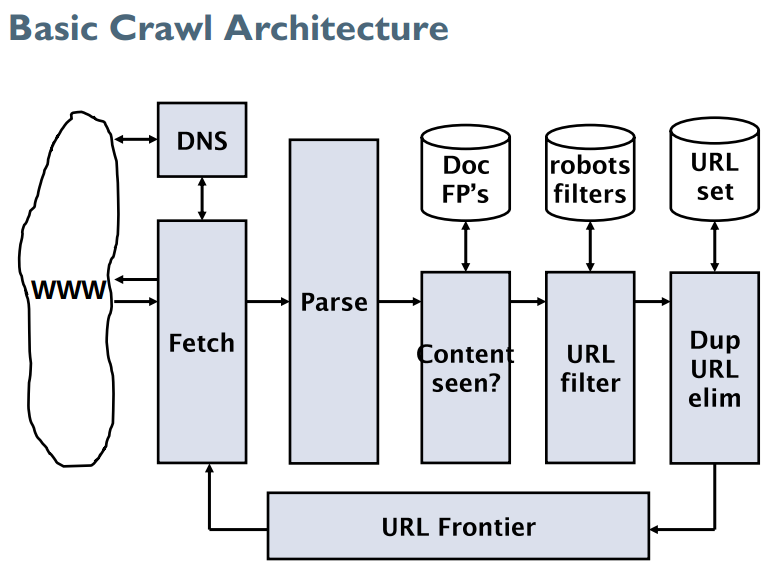
\includegraphics[width=0.7\linewidth]{./Media/basiccrawlarchitecture}
	\caption{Basic Crawl Architecture from Slides}
	\label{fig:basiccrawlarchitecture}
	\end{figure}
	
	It gets an url from the frontier, fetches the content if it can get past the `robots.txt' checker, checks if the content has already been seen, and adds it to the url filter after normalizing and checking if it does not already exist in the frontier or already visited urls.
	
	\subsection{Cut Corners}
	We could have used the Mercator scheme instead of just sleeping 1 second whenever the Crawler has finished with a page.
	
	The Crawler does find every url in the visited urls, but rather just the ones that are inside href attribute.
	
	The Crawler was limited to very few pages, 100-1000 primarily because the shingling with sketches is extremely slow for some reason.
	
	To actually check for content it might be a good idea to remove all the tags from the HTML content retrieved, but we do not do that.
	
	\section{Indexer}
	The indexer retrieves the items in the database, makes from the content, and makes features from those tokens using a stemmer and a stopword list. That feature is then added to the inverted index along with the id of the document.
	
	Adding to the inverted index works as such, it receives the term and the document id as mentioned, checks if the inverted index, which is a dictionary with a string key where the term is the key, and a posting list that contains a list of postings.
	
	If the inverted index does not already contained the term, it creates a list of postings, adds a posting with the document id, and adds that to inverted index using the term and a new posting list.
	
	If the inverted index does contain it, it checks if the document id already has a posting in that we might encounter the same word multiple times in the same document. It then sorts the postings.
	
	Otherwise it increments the frequency the term has been seen in the current document.
	
	And that's the construction of the inverted index which is really all that is needed for the index.
	
	\section{Ranker}
	For the ranker we used the cosine score.
		
	

\end{document}
